\documentclass{article}\usepackage[]{graphicx}\usepackage[]{color}
%% maxwidth is the original width if it is less than linewidth
%% otherwise use linewidth (to make sure the graphics do not exceed the margin)
\makeatletter
\def\maxwidth{ %
  \ifdim\Gin@nat@width>\linewidth
    \linewidth
  \else
    \Gin@nat@width
  \fi
}
\makeatother

\definecolor{fgcolor}{rgb}{0.345, 0.345, 0.345}
\newcommand{\hlnum}[1]{\textcolor[rgb]{0.686,0.059,0.569}{#1}}%
\newcommand{\hlstr}[1]{\textcolor[rgb]{0.192,0.494,0.8}{#1}}%
\newcommand{\hlcom}[1]{\textcolor[rgb]{0.678,0.584,0.686}{\textit{#1}}}%
\newcommand{\hlopt}[1]{\textcolor[rgb]{0,0,0}{#1}}%
\newcommand{\hlstd}[1]{\textcolor[rgb]{0.345,0.345,0.345}{#1}}%
\newcommand{\hlkwa}[1]{\textcolor[rgb]{0.161,0.373,0.58}{\textbf{#1}}}%
\newcommand{\hlkwb}[1]{\textcolor[rgb]{0.69,0.353,0.396}{#1}}%
\newcommand{\hlkwc}[1]{\textcolor[rgb]{0.333,0.667,0.333}{#1}}%
\newcommand{\hlkwd}[1]{\textcolor[rgb]{0.737,0.353,0.396}{\textbf{#1}}}%
\let\hlipl\hlkwb

\usepackage{framed}
\makeatletter
\newenvironment{kframe}{%
 \def\at@end@of@kframe{}%
 \ifinner\ifhmode%
  \def\at@end@of@kframe{\end{minipage}}%
  \begin{minipage}{\columnwidth}%
 \fi\fi%
 \def\FrameCommand##1{\hskip\@totalleftmargin \hskip-\fboxsep
 \colorbox{shadecolor}{##1}\hskip-\fboxsep
     % There is no \\@totalrightmargin, so:
     \hskip-\linewidth \hskip-\@totalleftmargin \hskip\columnwidth}%
 \MakeFramed {\advance\hsize-\width
   \@totalleftmargin\z@ \linewidth\hsize
   \@setminipage}}%
 {\par\unskip\endMakeFramed%
 \at@end@of@kframe}
\makeatother

\definecolor{shadecolor}{rgb}{.97, .97, .97}
\definecolor{messagecolor}{rgb}{0, 0, 0}
\definecolor{warningcolor}{rgb}{1, 0, 1}
\definecolor{errorcolor}{rgb}{1, 0, 0}
\newenvironment{knitrout}{}{} % an empty environment to be redefined in TeX

\usepackage{alltt}
\usepackage{natbib}



\IfFileExists{upquote.sty}{\usepackage{upquote}}{}
\begin{document}
\title{A Tale of Two Cities by Charles Dickens Wordcloud}
\author{Jorge Fitzmaurice}
\maketitle

\begin{abstract}
In this article we construct a wordcloud, using the tidytext R package, for Charles Dicken's Novel A Tale of Two Cities.


\end{abstract}

\textit{A Tale of Two Cities} (1859)\footnote{The novel was published by Charles Dickens.} is a novel by Charles Dickens, set in London and Paris before and during the French Revolution. The novel tells the story of the French Doctor Manette, his 18-year-long imprisonment in the Bastille in Paris and his release to life in London with his daughter Lucie, whom he had never met; Lucie's marriage and the collision between her beloved husband and the people who caused her father's imprisonment; and Monsieur and Madame Defarge, sellers of wine in a poor suburb of Paris. The story is set against the conditions that led up to the French Revolution and the Reign of Terror.

\section{The Gutenbergr Package}
There is a relatively new package for R, guntenbergr, that gives one access to a variety of public domain works from the Project Gutenberg collection\citep{Silge}.  One first has to install this package and bring it in with library.  You may then call the following function to find the title number and then call the next function to download the document and store the result.  The result will be a data frame.

\begin{knitrout}
\definecolor{shadecolor}{rgb}{0.969, 0.969, 0.969}\color{fgcolor}\begin{kframe}
\begin{alltt}
\hlkwd{library}\hlstd{(gutenbergr)}
\end{alltt}


{\ttfamily\noindent\color{warningcolor}{\#\# Warning: package 'gutenbergr' was built under R version 3.4.2}}\begin{alltt}
\hlkwd{gutenberg_works}\hlstd{(title}\hlopt{==}\hlstr{'A Tale of Two Cities'}\hlstd{)}
\end{alltt}
\begin{verbatim}
## # A tibble: 1 x 8
##   gutenberg_id                title           author gutenberg_author_id
##          <int>                <chr>            <chr>               <int>
## 1           98 A Tale of Two Cities Dickens, Charles                  37
## # ... with 4 more variables: language <chr>, gutenberg_bookshelf <chr>,
## #   rights <chr>, has_text <lgl>
\end{verbatim}
\begin{alltt}
\hlstd{dickens}\hlkwb{<-}\hlkwd{gutenberg_download}\hlstd{(}\hlnum{98}\hlstd{)}

\hlstd{dickens}
\end{alltt}
\begin{verbatim}
## # A tibble: 15,865 x 2
##    gutenberg_id                             text
##           <int>                            <chr>
##  1           98             A TALE OF TWO CITIES
##  2           98                                 
##  3           98 A STORY OF THE FRENCH REVOLUTION
##  4           98                                 
##  5           98               By Charles Dickens
##  6           98                                 
##  7           98                                 
##  8           98                         CONTENTS
##  9           98                                 
## 10           98                                 
## # ... with 15,855 more rows
\end{verbatim}
\end{kframe}
\end{knitrout}

This dataframe has two columns, one for each line in Charles Dicken's Novel, and one indicating the gutenberg ID from which the book came from.  Let's first unnest the lines to get every word in the novel in a different row:

\begin{knitrout}
\definecolor{shadecolor}{rgb}{0.969, 0.969, 0.969}\color{fgcolor}\begin{kframe}
\begin{alltt}
\hlkwd{library}\hlstd{(tidytext)}
\hlkwd{library}\hlstd{(dplyr)}
\hlstd{dickens_words}\hlkwb{<-}\hlstd{dickens}\hlopt
                  \hlkwd{unnest_tokens}\hlstd{(word,text)}
\hlstd{dickens_words}\hlopt{$}\hlstd{gutenberg_id}\hlkwb{<-}\hlkwa{NULL}
\hlkwd{head}\hlstd{(dickens_words)}
\end{alltt}
\begin{verbatim}
## # A tibble: 6 x 1
##     word
##    <chr>
## 1      a
## 2   tale
## 3     of
## 4    two
## 5 cities
## 6      a
\end{verbatim}
\end{kframe}
\end{knitrout}

\noindent Now we are ready to get the sentiments data frame.

\section{The Sentiments Data Frame}

The sentiments data frame is part of the tidy text package and it gives us different lexicons to work with. For this article the NRC lexicon will be used. The NRC lexicon give us the emotion represented by certain word.
For this article, we will only be using the fear words in the NRC lexicon for the first wordcloud and the joy words in the NRC lexicon for the second wordcloud.

\begin{knitrout}
\definecolor{shadecolor}{rgb}{0.969, 0.969, 0.969}\color{fgcolor}\begin{kframe}
\begin{alltt}
\hlstd{nrc}\hlkwb{<-}\hlkwd{get_sentiments}\hlstd{(}\hlstr{'nrc'}\hlstd{)}
\hlkwd{unique}\hlstd{(nrc}\hlopt{$}\hlstd{sentiment)}
\end{alltt}
\begin{verbatim}
##  [1] "trust"        "fear"         "negative"     "sadness"     
##  [5] "anger"        "surprise"     "positive"     "disgust"     
##  [9] "joy"          "anticipation"
\end{verbatim}
\begin{alltt}
\hlstd{fear_words}\hlkwb{<-}\hlstd{nrc}\hlopt
            \hlkwd{filter}\hlstd{(sentiment} \hlopt{==} \hlstr{'fear'}\hlstd{)}
\hlkwd{head}\hlstd{(fear_words)}
\end{alltt}
\begin{verbatim}
## # A tibble: 6 x 2
##          word sentiment
##         <chr>     <chr>
## 1     abandon      fear
## 2   abandoned      fear
## 3 abandonment      fear
## 4   abduction      fear
## 5       abhor      fear
## 6   abhorrent      fear
\end{verbatim}
\begin{alltt}
\hlstd{joy_words}\hlkwb{<-}\hlstd{nrc}\hlopt
  \hlkwd{filter}\hlstd{(sentiment} \hlopt{==} \hlstr{'joy'}\hlstd{)}
\hlkwd{head}\hlstd{(joy_words)}
\end{alltt}
\begin{verbatim}
## # A tibble: 6 x 2
##            word sentiment
##           <chr>     <chr>
## 1    absolution       joy
## 2     abundance       joy
## 3      abundant       joy
## 4      accolade       joy
## 5 accompaniment       joy
## 6    accomplish       joy
\end{verbatim}
\end{kframe}
\end{knitrout}

Next, we would like to join the data frame with the words for the novel and the data frame with the sentiments words to keep only those words that are represented in the sentiment lexicon with the selected sentiments.

\section{The Wordcloud}
To make the wordcloud, we first have to join the two data frames to get a new data frame with only the words with the appropriate sentiment are in there. We can use a function from the dplyr package for this:

\begin{knitrout}
\definecolor{shadecolor}{rgb}{0.969, 0.969, 0.969}\color{fgcolor}\begin{kframe}
\begin{alltt}
\hlstd{dickens_fear}\hlkwb{<-}\hlkwd{inner_join}\hlstd{(dickens_words,fear_words)}
\end{alltt}


{\ttfamily\noindent\itshape\color{messagecolor}{\#\# Joining, by = "{}word"{}}}\begin{alltt}
\hlstd{dickens_fear}
\end{alltt}
\begin{verbatim}
## # A tibble: 3,009 x 2
##          word sentiment
##         <chr>     <chr>
##  1 revolution      fear
##  2     honest      fear
##  3       plea      fear
##  4       fire      fear
##  5   darkness      fear
##  6        die      fear
##  7   darkness      fear
##  8    despair      fear
##  9       evil      fear
## 10      ghost      fear
## # ... with 2,999 more rows
\end{verbatim}
\begin{alltt}
\hlstd{dickens_joy}\hlkwb{<-}\hlkwd{inner_join}\hlstd{(dickens_words,joy_words)}
\end{alltt}


{\ttfamily\noindent\itshape\color{messagecolor}{\#\# Joining, by = "{}word"{}}}\begin{alltt}
\hlstd{dickens_joy}
\end{alltt}
\begin{verbatim}
## # A tibble: 2,638 x 2
##              word sentiment
##             <chr>     <chr>
##  1 congratulatory       joy
##  2      companion       joy
##  3         honest       joy
##  4        triumph       joy
##  5           hope       joy
##  6        present       joy
##  7           good       joy
##  8        blessed       joy
##  9       birthday       joy
## 10        spirits       joy
## # ... with 2,628 more rows
\end{verbatim}
\end{kframe}
\end{knitrout}

Now, we need to calculate the frequencies of the words in the novel.  Again, we can use standard dplyr techniques for this:

\begin{knitrout}
\definecolor{shadecolor}{rgb}{0.969, 0.969, 0.969}\color{fgcolor}\begin{kframe}
\begin{alltt}
\hlstd{fear_freq}\hlkwb{<-}\hlstd{dickens_fear}\hlopt
                  \hlkwd{group_by}\hlstd{(word)}\hlopt
                  \hlkwd{summarize}\hlstd{(}\hlkwc{count}\hlstd{=}\hlkwd{n}\hlstd{())}
\hlstd{fear_freq}
\end{alltt}
\begin{verbatim}
## # A tibble: 583 x 2
##           word count
##          <chr> <int>
##  1     abandon     1
##  2   abandoned    10
##  3 abandonment     1
##  4  abominable     2
##  5     absence     8
##  6       abuse     1
##  7       abyss     1
##  8    accident     3
##  9  accidental     3
## 10    accursed     5
## # ... with 573 more rows
\end{verbatim}
\begin{alltt}
\hlstd{joy_freq}\hlkwb{<-}\hlstd{dickens_joy}\hlopt
                  \hlkwd{group_by}\hlstd{(word)}\hlopt
                  \hlkwd{summarize}\hlstd{(}\hlkwc{count}\hlstd{=}\hlkwd{n}\hlstd{())}
\hlstd{joy_freq}
\end{alltt}
\begin{verbatim}
## # A tibble: 335 x 2
##             word count
##            <chr> <int>
##  1     abundance     1
##  2      abundant     4
##  3 accompaniment     2
##  4  accomplished     5
##  5       achieve     1
##  6   achievement     1
##  7     admirable     4
##  8    admiration     5
##  9      adorable     1
## 10       advance    10
## # ... with 325 more rows
\end{verbatim}
\end{kframe}
\end{knitrout}



Finally, it's time to generate the wordcloud for the fear words:

\begin{knitrout}
\definecolor{shadecolor}{rgb}{0.969, 0.969, 0.969}\color{fgcolor}\begin{kframe}
\begin{alltt}
\hlkwd{library}\hlstd{(wordcloud)}
\hlkwd{wordcloud}\hlstd{(fear_freq}\hlopt{$}\hlstd{word,fear_freq}\hlopt{$}\hlstd{count,}\hlkwc{min.freq}\hlstd{=}\hlnum{5}\hlstd{)}
\end{alltt}
\end{kframe}
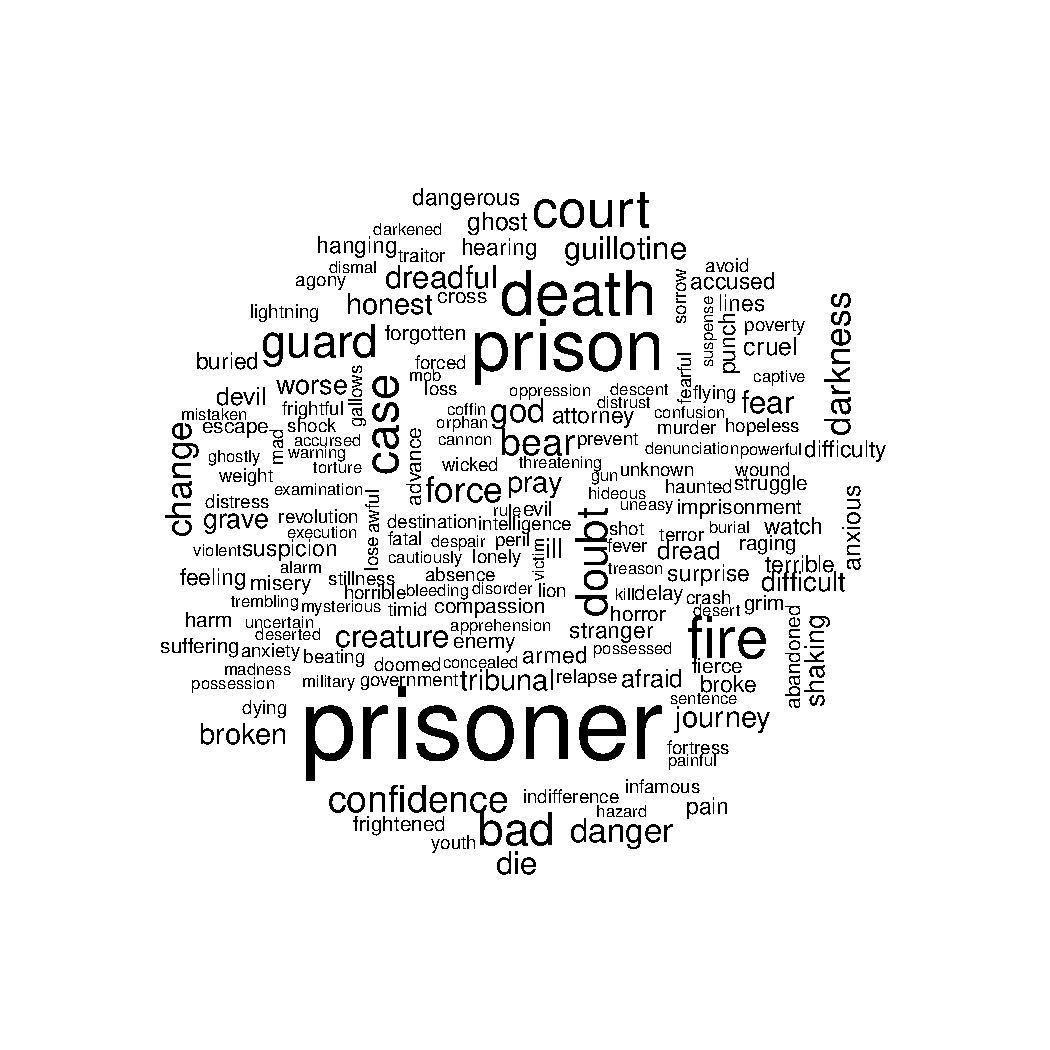
\includegraphics[width=\maxwidth]{figure/unnamed-chunk-7-1} 

\end{knitrout}

Lastly, it's time to generate the wordcloud for the joy words:

\begin{knitrout}
\definecolor{shadecolor}{rgb}{0.969, 0.969, 0.969}\color{fgcolor}\begin{kframe}
\begin{alltt}
\hlkwd{wordcloud}\hlstd{(joy_freq}\hlopt{$}\hlstd{word,joy_freq}\hlopt{$}\hlstd{count,}\hlkwc{min.freq}\hlstd{=}\hlnum{3}\hlstd{)}
\end{alltt}
\end{kframe}
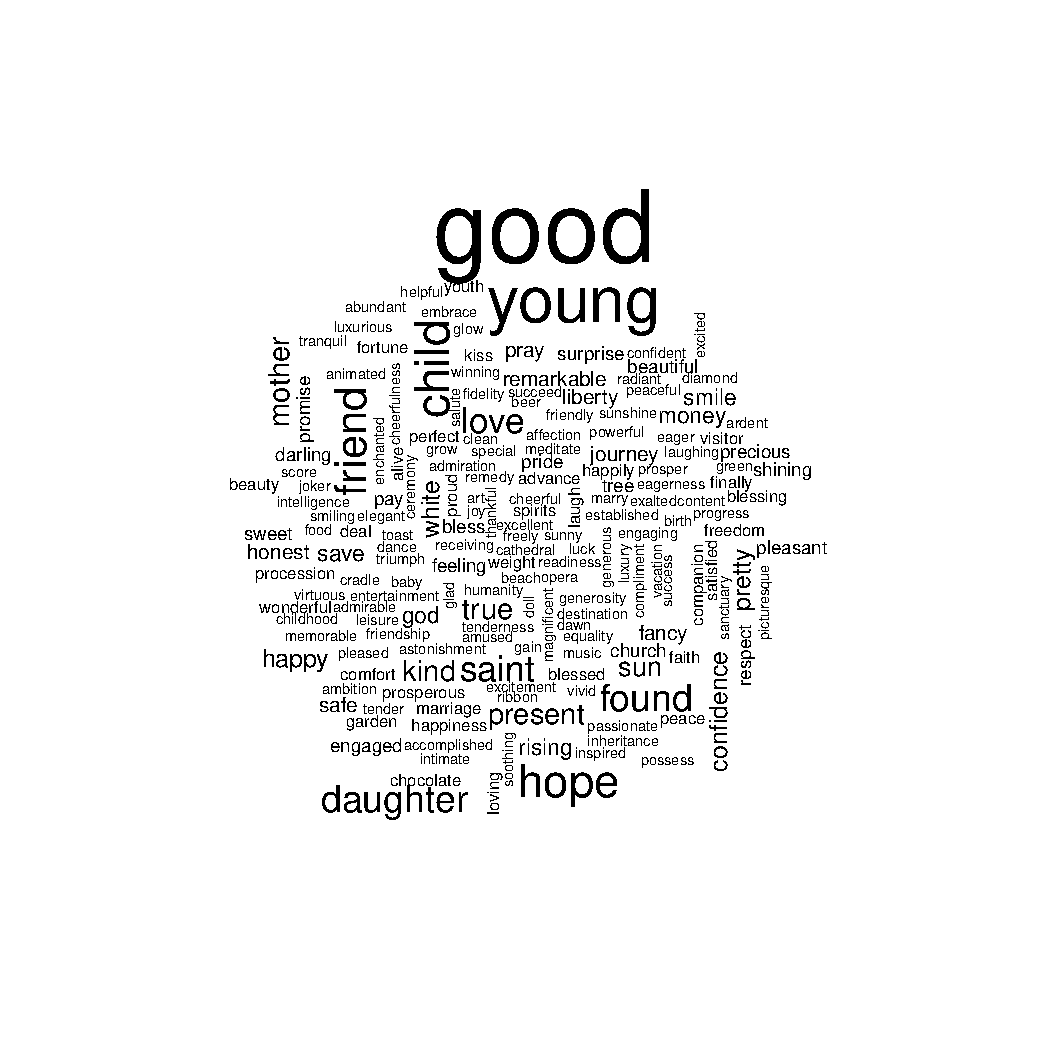
\includegraphics[width=\maxwidth]{figure/unnamed-chunk-8-1} 

\end{knitrout}

\bibliographystyle{apa}
\bibliography{packages}
\nocite{*}



\end{document}
